\begin{center}
Problema F

Quero imprimir em 3D!

{\tiny Por Douglas Cedrim}

Timelimit: $1$	
\end{center}

{\footnotesize
	Impressão 3D é uma tecnologia arretada, que está em alta, e que possibilita imprimir uma peça tridimensional utilizando: um modelo digital devidamente processado e um \emph{filamento} plástico - que irá constituir o material da peça impressa. A ideia geral é que um modelo digital (modelo original) seja convertido em uma versão do modelo fatiado ao longo do eixo Z, e a impressora 3D irá depositar filamento, de baixo para cima, uma fatia por vez, uma sobre a outra, ao longo de planos paralelos ao plano XY, seguindo o caminho dos contornos do objeto e de seu interior, que é definido pelo \emph{padrão de preenchimento}.
	%e se deslocando ao longo de planos paralelos ao plano XZ. 
	
	Na Figura~\ref{fig:f_fatias} esse processo é ilustrado de forma que cada fatia ($h$) está representada em vermelho, com um padrão de preenchimento (quadriláteros) representado em laranja. Note que outros padrões de preenchimento podem ser usados. Assim, o total de filamento na fatia corresponde à combinação desse caminho formado pelas cores vermelha e laranja. Na Figura~\ref{fig:f_imp}, por exemplo, é ilustrado todo o sistema mostrando o filamento e a peça impressa, com um total de 6 fatias ($h=6$).
	
	\begin{figure}[ht]
		\begin{subfigure}[ht]{0.7\textwidth}
			\centering
			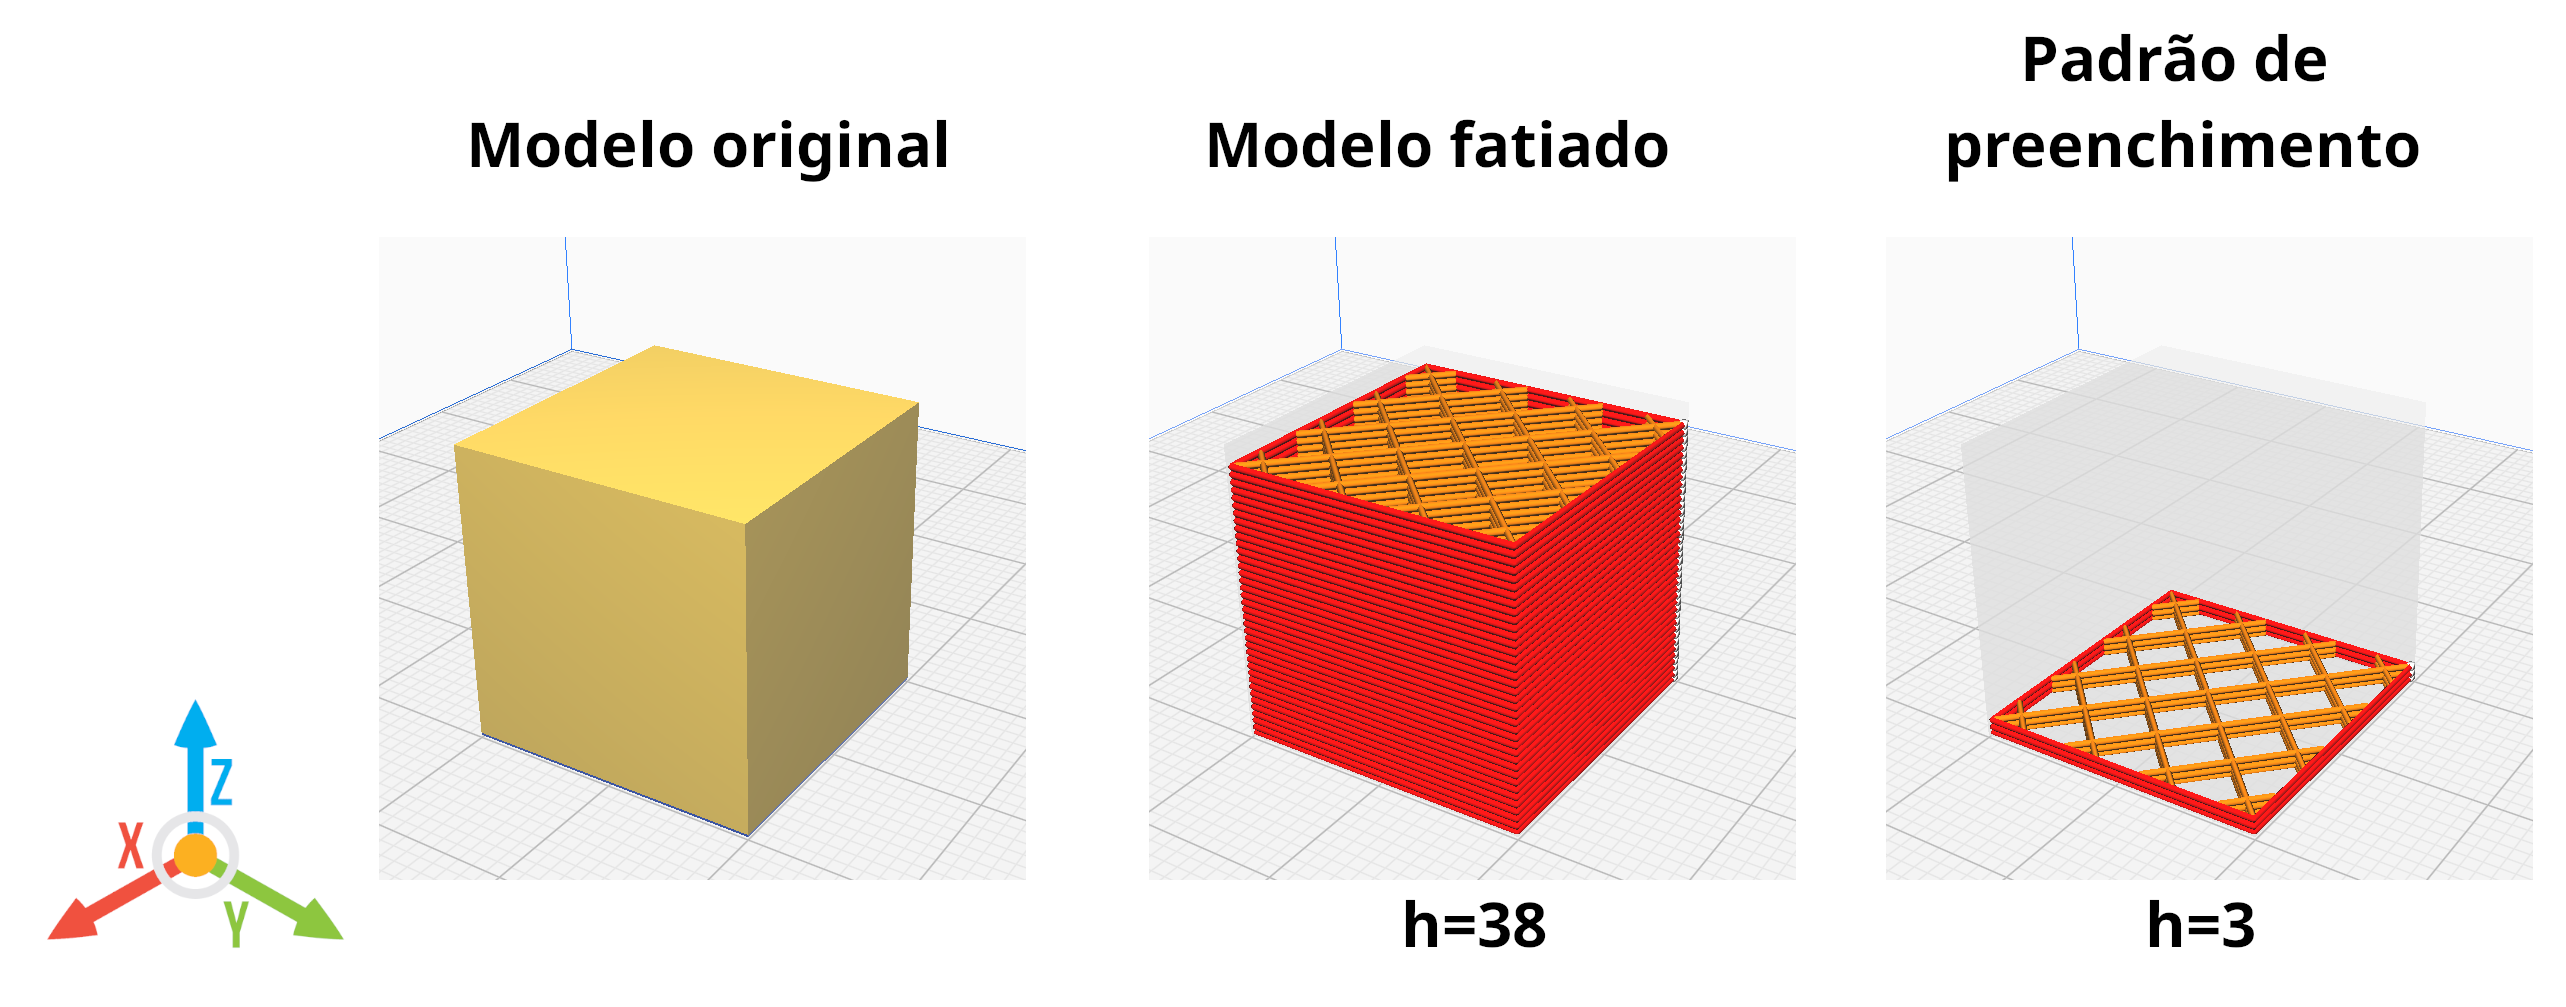
\includegraphics[width=\linewidth]{fig/f_fig3.png}
			\caption{Fatiamento de um modelo 3D.}
			\label{fig:f_fatias}
		\end{subfigure}
		\hfill
		\begin{subfigure}[ht]{0.35\textwidth}
			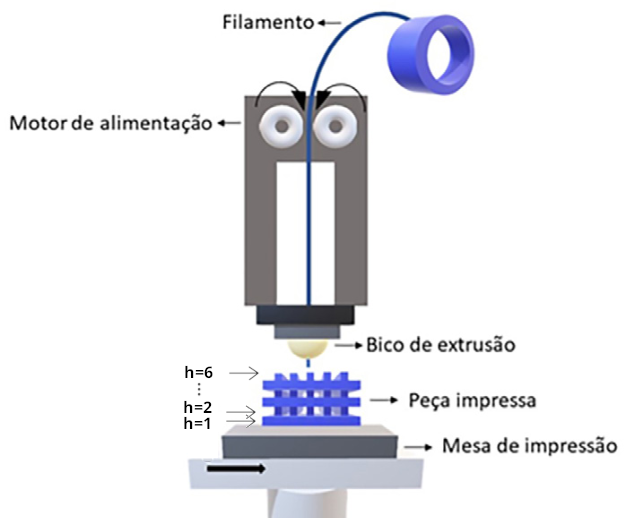
\includegraphics[width=\linewidth]{fig/f_fig2.png}
			\caption{Fig. adaptada de [1].}
			\label{fig:f_imp}
		\end{subfigure}
		\caption{Impressão 3D.}
	\end{figure}
	
	O professor Márcio Belo recebeu alguns modelos digitais %$\{M\}$
	já fatiados, e com um número fixo de fatias diferente para cada modelo ($h_{max}$). Ele precisa calcular o quanto de filamento ele irá necessitar para efetuar a impressão de cada modelo. 
	%
	Para ajudá-lo você deverá estimar o quanto precisará de filamento em cada fatia $h$ e então calcular o montante para o modelo inteiro. Para simplificar, dado um modelo $M$, todas as suas fatias são iguais e vão consumir a mesma quantidade de filamento. Além disso, considere também que o montante de filamento que pode ser depositado entre fatias subsequentes é irrisório, irrelevante para sua estimativa. O comprimento de filamento consumido por unidade de comprimento de impressão é igual.
	
	Para um modelo $M$ você terá disponível um conjunto de vértices $V=\{v_i\}_{i=1}^n$, ordenados no sentido anti-horário, com coordenadas $(x_i, y_i)$  que definem o contorno externo da fatia como um polígono convexo. O seu padrão de preenchimento deverá ser triangular, análogo à triangulação $\mathcal{T}$ ilustrada em vermelho na Figura~\ref{fig:tri}, de forma que sempre o primeiro vértice $v_1$ é comum a todos os triângulos. Assim, os vértices de qualquer triângulo $t \in \mathcal{T}$ estarão contidos em $\{v_i\}$. 
	
	Para fins de otimização do uso do filamento, a impressora está configurada para não passar pela mesma aresta mais de uma vez.
	
	\begin{figure}[ht]
		\centering
		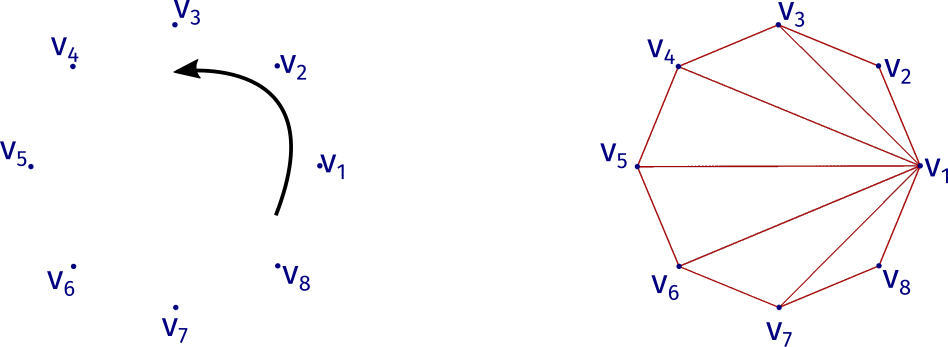
\includegraphics[width=10cm]{fig/f_disco_tri.png}
		\caption{Triangulação $\mathcal{T}$ de um modelo $M$.}
		\label{fig:tri}
	\end{figure}

	\textbf{[1]} BERNARDO, Marcela Piassi et al. \textit{Processamento e aplicação de biomateriais poliméricos: avanços recentes e perspectivas}. Química Nova, v. 44, p. 1311-1327, 2021.
	

%	\begin{figure}[h]
%		\centering
%		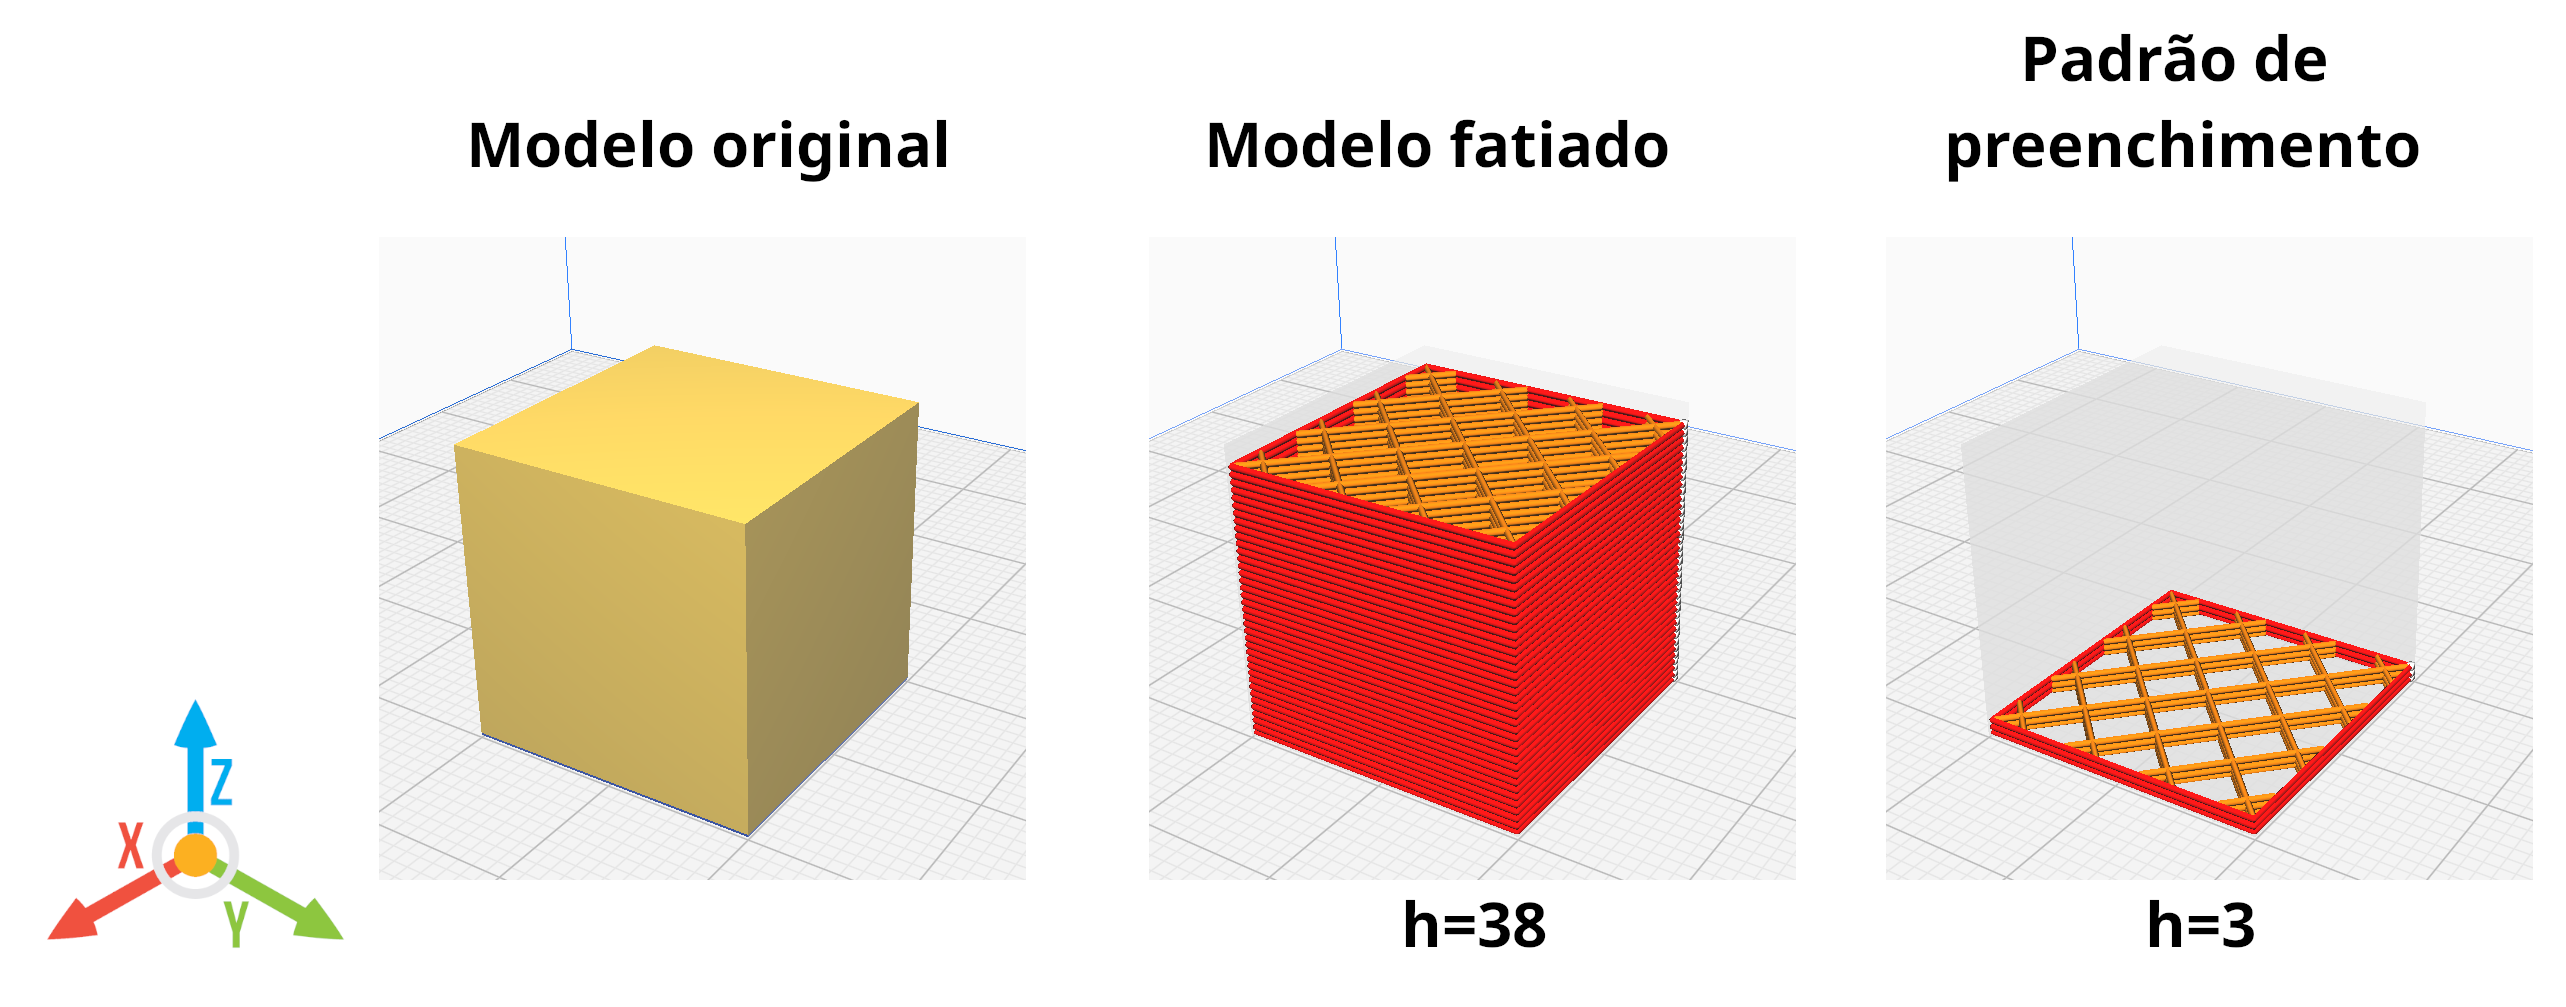
\includegraphics[width=13cm]{fig/f_fig3.png}
%		\caption{Fatiamento de um modelo 3D.}
%		\label{fig:f_fatias}
%	\end{figure}
	
%	O processo funciona da seguinte forma: 	um motor puxa o filamento até um bico de extrusão, onde o filamento plástico é aquecido e muda sua consistência passando a ficar um pouco fluido. O bico começa a se movimentar na horizontal ao longo da mesa de impressão, passando por cada 

%	\begin{figure}[h]
%		\centering
%		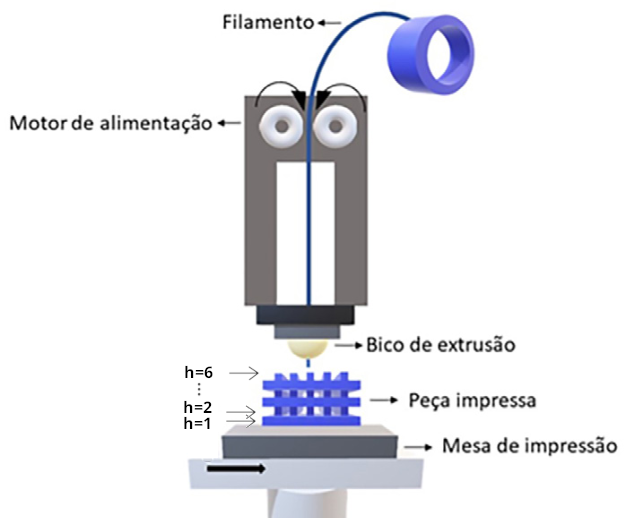
\includegraphics[width=7cm]{fig/f_fig2.png}
%		\caption{Exemplo de um processo de impressão 3D. Figura adaptada de .}
%		\label{fig:f_impressao}
%	\end{figure}
%	
%	A partir disso o bico ... . A Figura~\ref{fig:f_impressao} ilustra o processo com com uma peça contendo \textbf{6 níveis} de altura (h=6).



	

%Uma vez que uma camada é solidificada, a mesa é movimentada uma camada para baixo. A camada subsequente é depositada sobre a mesa por um rolo, e o processo é repetido até que todo o objeto seja formado


\vspace{0.3cm}
\textbf{Entrada}
Cada entrada contém os dados do modelo M fatiado. A primeira linha contém a quantidade de fatias do modelo $h_{max}$. A segunda linha contém o número de vértices $n$, com $(3 \leq n \leq 10^2)$. A terceira linha é formada pela sequência de vértices na forma de suas coordenadas $x_i, y_i$, com cada coordenada representada em ponto flutuante, com precisão de três casas decimais.

% A primeira linha contém um inteiro $X$ indicando o nível (iniciado em 0) da hierarquia onde estão os genes $(0 \leq X \leq 99)$. A segunda linha representa a quantidade $N$ de genes de um indivíduo $(1 \leq X \leq 100)$. A terceira linha é formada pela sequência de genes de um indivíduo, sendo que cada elemento está no intervalo de $0$ a $10000$.

\vspace{0.3cm}
\textbf{Saída}
O sistema deve retornar o montante total de filamento necessário para impressão do modelo M como um número inteiro. Para isso, efetue o arredondamento apenas ao final das contas, para o menor número inteiro maior ou igual que o montante. 

%O sistema deve retornar a sequência de genes significativos seguido do caractere \#, todos separados por um único espaço, conforme o nível hierárquico $X$, indicado na primeira linha da entrada. Os filhos 1, 2, 3 e 4, devem ser representados da esquerda para direta. Se nenhum gene significativo for encontrado no nível indicado, a saída terá apenas o caractere \#.

\begin{table}[ht]
    \centering
   % \small
    \begin{tabular}{|p{12cm}|p{3cm}|}
        \hline
        \begin{center}
            \vspace{-0.3cm}
            \textbf{Exemplos de Entrada}
            \vspace{-0.3cm}
        \end{center} 
         &  
        \begin{center}
            \vspace{-0.3cm}
            \textbf{Exemplos de Saída}
            \vspace{-0.3cm}
        \end{center} \\ \hline
		    \texttt{16} & \texttt{226} \\
		    \texttt{4} & \texttt{} \\
		    \texttt{0.0 0.0 4.0 0.0 4.0 1.0 0.0 1.0} & \texttt{}\\
         \hline
		    \texttt{85} & \texttt{1494} \\
			\texttt{10} & \texttt{} \\
			\texttt{1.000 0.000 0.809 0.588 0.309 0.951 -0.309 0.951 -0.809 0.588 -1.000 0.000 -0.809 -0.588 -0.309 -0.951 0.309 -0.951 0.809 -0.588} & \texttt{}\\
         \hline    
            \texttt{32} & \texttt{1998} \\
        	\texttt{16} & \texttt{} \\
        	\texttt{3.000 0.000 2.772 0.383 2.121 0.707 1.148 0.924 0.000 1.000 -1.148 0.924 -2.121 0.707 -2.772 0.383 -3.000 0.000 -2.772 -0.383 -2.121 -0.707 -1.148 -0.924 -0.000 -1.000 1.148 -0.924 2.121 -0.707 2.772 -0.383} & \texttt{}\\
%         \hline    
         %\texttt{2} & \texttt{2501 25 38 78 \#} \\  
         %\texttt{10} & \texttt{} \\  
         %\texttt{5 98 78 50 7 38 25 61 1579 2501} & \texttt{} \\
         \hline    
    \end{tabular}
    \caption{Exemplos de entradas e saídas}
    \label{tab:inputH}
\end{table}}

%\normalsize


\newpage

\begin{center}
\noindent
\lstinputlisting{abobora_23/F/F3.cpp}
\end{center}